\documentclass[12pt]{report}
\usepackage[utf8]{inputenc}
\usepackage[russian]{babel}
%\usepackage[14pt]{extsizes}
\usepackage{listings}

% Для листинга кода:
\lstset{ %
language=python,                 % выбор языка для подсветки (здесь это Python)
basicstyle=\small\sffamily, % размер и начертание шрифта для подсветки кода
numbers=left,               % где поставить нумерацию строк (слева\справа)
numberstyle=\tiny,           % размер шрифта для номеров строк
stepnumber=1,                   % размер шага между двумя номерами строк
numbersep=5pt,                % как далеко отстоят номера строк от подсвечиваемого кода
showspaces=false,            % показывать или нет пробелы специальными отступами
showstringspaces=false,      % показывать или нет пробелы в строках
showtabs=false,             % показывать или нет табуляцию в строках
frame=single,              % рисовать рамку вокруг кода
tabsize=2,                 % размер табуляции по умолчанию равен 2 пробелам
captionpos=t,              % позиция заголовка вверху [t] или внизу [b] 
breaklines=true,           % автоматически переносить строки (да\нет)
breakatwhitespace=false, % переносить строки только если есть пробел
escapeinside={\#*}{*)}   % если нужно добавить комментарии в коде
}

% Для измененных титулов глав:
\usepackage{titlesec, blindtext, color} % подключаем нужные пакеты
\definecolor{gray75}{gray}{0.75} % определяем цвет
\newcommand{\hsp}{\hspace{20pt}} % длина линии в 20pt
% titleformat определяет стиль
\titleformat{\chapter}[hang]{\Huge\bfseries}{\thechapter\hsp\textcolor{gray75}{|}\hsp}{0pt}{\Huge\bfseries}


% plot
\usepackage{pgfplots}
\usepackage{filecontents}
\usetikzlibrary{datavisualization}
\usetikzlibrary{datavisualization.formats.functions}
\begin{filecontents}{bubble.dat}
20	   0.0034351         
50          0.0244715          
80          0.0444493           
100          0.0678084          
\end{filecontents}

\begin{filecontents}{insertion.dat}
20          0.0010774            
50          0.0066717          
80          0.0133443        
100          0.0193913          
\end{filecontents}

\begin{filecontents}{quicksort.dat}
20           0.0012343        
50           0.0050528           
80           0.0057573          
100           0.0075033           
\end{filecontents}




\setcounter{tocdepth}{5}
\begin{document}

%\def\chaptername{} % убирает "Глава"
\begin{titlepage}

	\fontsize{12pt}{12pt}\selectfont
	\noindent \begin{minipage}{0.15\textwidth}
		
\includegraphics[width=\linewidth]{b_logo.jpg}
	\end{minipage}
	\noindent\begin{minipage}{0.9\textwidth}\centering
		\textbf{Министерство науки и высшего образования Российской Федерации}\\
		\textbf{Федеральное государственное бюджетное образовательное учреждение высшего образования}\\
		\textbf{«Московский государственный технический университет имени Н.Э.~Баумана}\\
		\textbf{(национальный исследовательский университет)»}\\
		\textbf{(МГТУ им. Н.Э.~Баумана)}
	\end{minipage}
	
	\noindent\rule{18cm}{3pt}
	\newline\newline
	\noindent ФАКУЛЬТЕТ $\underline{\textbf{«Информатика и системы управления»}}$ \newline\newline
	\noindent КАФЕДРА $\underline{\textbf{«Программное обеспечение ЭВМ и информационные технологии»}}$\newline\newline\newline\newline\newline\newline\newline
	
	
	\begin{center}
		\Large\textbf{Отчет по лабораторной работе №3 по курсу <<Анализ алгоритмов>>}
	\end{center}
	
	\noindent\textbf{Тема} $\underline{\textbf{Алгоритмы сортировки~~~~~~~~~~~~~~~~~~~~~~~~~~~}}$\newline\newline\newline
	\noindent\textbf{Студент} $\underline{\textbf{Челядинов И.Д.~~~~~~~~~~~~~~~~~~~~~~~~~~~~~~~~~}}$\newline\newline
	\noindent\textbf{Группа} $\underline{\textbf{ИУ7-53Б~~~~~~~~~~~~~~~~~~~~~~~~~~~~~~~~~~~~~~~~~~~~}}$\newline\newline
	\noindent\textbf{Оценка (баллы)} $\underline{\textbf{~~~~~~~~~~~~~~~~~~~~~~~~~~~~~~~~~~~~~~~~~~}}$\newline\newline
	\noindent\textbf{Преподаватели} $\underline{\textbf{Волкова Л.Л., Строганов Ю.В.}}$\newline
	
	\begin{center}
		\vfill
		Москва~---~\the\year
		~г.
	\end{center}
 \restoregeometry
\end{titlepage}

\setcounter{page}{2}
\tableofcontents

\newpage
\chapter*{Введение}
\addcontentsline{toc}{chapter}{Введение}

\textbf{Сортировкой, или упорядочением массива} называется расположение его элементов по возрастанию (или убыванию) ~\cite{one}. Для решения задачи сортировки было разработано множество алгоритмов, различающихся по трудоемкости и эффективности в связи с затрачиваемыми ими ресурсами ЭВМ. К таким алгоритмам относятся сортировка пузырьком, сортировка вставками, сортировка выбором, сортировка Шелла, сортировка расческой, быстрая сортировка и многие другие.

В рамках этой лабораторной работы будут рассмотрены следующие алгоритмы сортировки: сортировка пузырьком,  сортировка вставками и быстрая сортировка.

Целью данной лабораторной работы является изучение, реализация и сравнительный анализ алгоритмов сортировки массивов. 

В данной лабораторной работе требуется решить пять задач.
\begin{enumerate}
\item Изучить и программно реализовать алгоритм сортировки пузырьком;
\item Изучить и программно реализовать алгоритм сортировки вставками;
\item Изучить и программно реализовать алгоритм быстрой сортировки;
\item Оценить трудоемкость вышеперечисленных алгоритмов;
\item Сделать сравнительный анализ по затрачиваемым ресурсам (времени) компьютера на реализацию каждого рассмотренного алгоритма.
\end{enumerate}
Критерии оценки эффективности алгоритма.
\begin{enumerate}
\item Количество шагов алгоритма, необходимых для упорядочения.
\item Количество сравнений элементов.
\item Количество перестановок, выполняемых при сортировке.
\end{enumerate}
\chapter{Аналитическая часть}
 В данном разделе будут показаны теоретические сведения о каждом алгоритме, их преимущества и недостатки.

 \section{Сортировка пузырьком}

 \textbf{Сортировка пузырьком} - это сортировка, в которой обходим массив от начала до конца, попутно меняя местами неотсортированные соседние элементы. В результате первого прохода на последнее место «всплывёт» максимальный элемент. Теперь снова обходим неотсортированную часть массива (от первого элемента до предпоследнего) и меняем по пути неотсортированных соседей. Данный алгоритм не применяется на практике из-за низкой эффективности. ~\cite{two}
 
 \section{Сортировка вставками}
 \textbf{Сортировка вставками} - алгоритм сортировки, в котором элементы входной последовательности просматриваются по одному, и каждый новый поступивший элемент размещается в подходящее место среди ранее упорядоченных элементов. ~\cite{free} 
 
 На рисунке \ref{fg:ref1} представлен пример сортировки вставками.
\begin{figure}[ht!]
	\centering{
		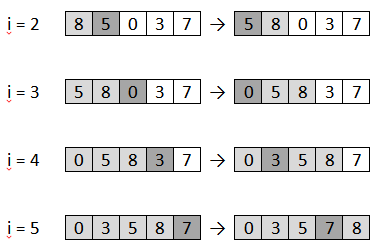
\includegraphics[scale=0.8]{insert.jpg}
		\caption{Пример сортировки вставками}
		\label{fg:ref1}}
\end{figure}
\newpage
 \section{Быстрая сортировка}
 \textbf{Быстрая сортировка} - представляет собой усовершенствованный метод сортировки, основанный на принципе обмена  ~\cite{four}.

Основные шаги алгоритма:
\begin{enumerate}
\item Выбрать из массива элемент, называемый опорным. Это может быть любой из элементов массива. От выбора опорного элемента не зависит корректность алгоритма, но в отдельных случаях может сильно зависеть его эффективность ~\cite{five}.  
\item Сравнить все остальные элементы с опорным и переставить их в массиве так, чтобы разбить массив на три непрерывных отрезка, следующих друг за другом: «элементы меньшие опорного», «равные» и «большие».
\item Для отрезков «меньших» и «больших» значений выполнить рекурсивно ту же последовательность операций, если длина отрезка больше единицы.
\end{enumerate}

\section{Вывод}
В данном разделе приведены основные принципы каждого алгоритма сортировок. Указано, что необходимо сделать для сортировки.

\chapter{Конструкторская часть}
В данной части будут приведены схемы алгоритма сортировки пузырьком, вставкой и схема быстрой сортировки.
\section{Сортировка пузырьком}
На рисунке 2.1 представлена схема алгоритма сортировки пузырьком.
\begin{center}
		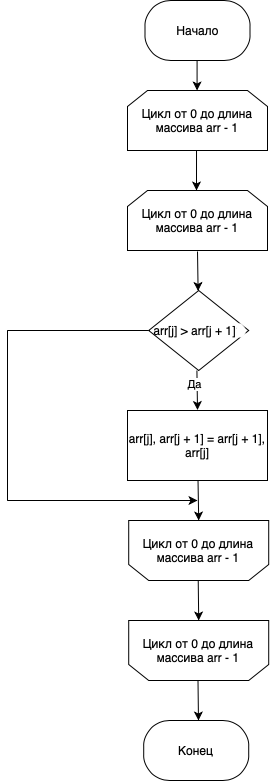
\includegraphics[scale=0.8]{BubbleSort.png}
		
			Рис 2.1: Схема алгоритма сортировки пузырьком
\end{center}

\section{Сортировка вставками}

На рисунке 2.2 представлена схема алгоритма сортировки вставками.

\begin{center}
		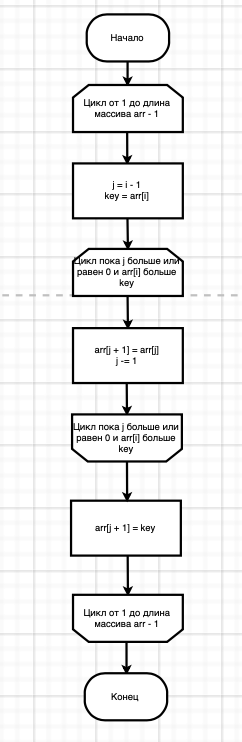
\includegraphics[scale=1.2]{InsertSort.png}
		
			Рис 2.2: Схема алгоритма сортировки вставками
\end{center}

\section{Быстрая сортировка}

На рисунках 2.3 - 2.4 - 2.5 представлена схема алгоритма быстрой сортировки.

\begin{center}
		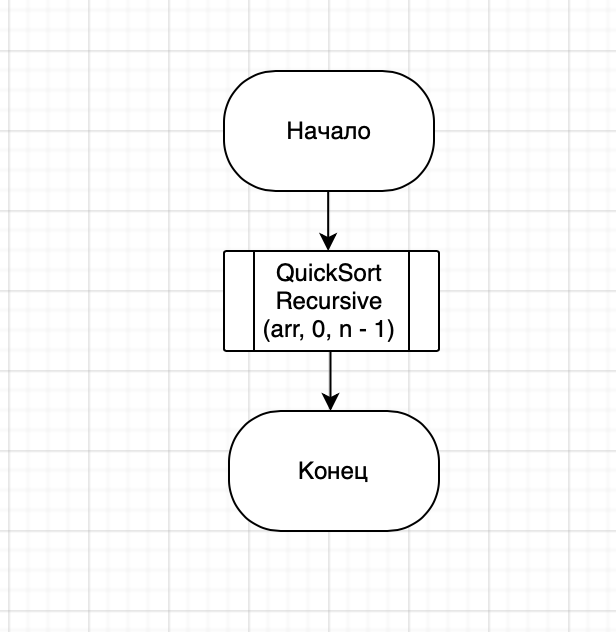
\includegraphics[scale=0.8]{QuickSort.png}
		
			Рис 2.3: Схема алгоритма быстрой сортировки (часть 1)
\end{center}

\begin{center}
		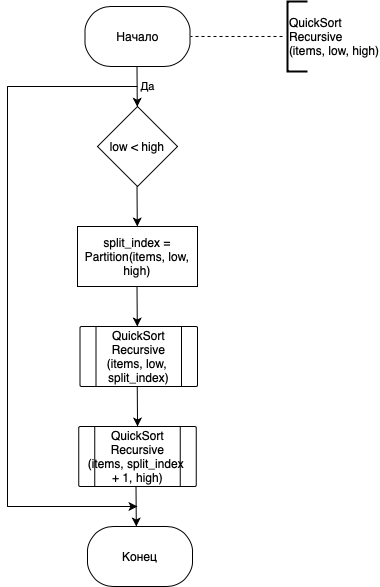
\includegraphics[scale=1.1]{QuickSortRec.png}
		
			Рис 2.4: Схема алгоритма быстрой сортировки (часть 2)
\end{center}

\begin{center}
		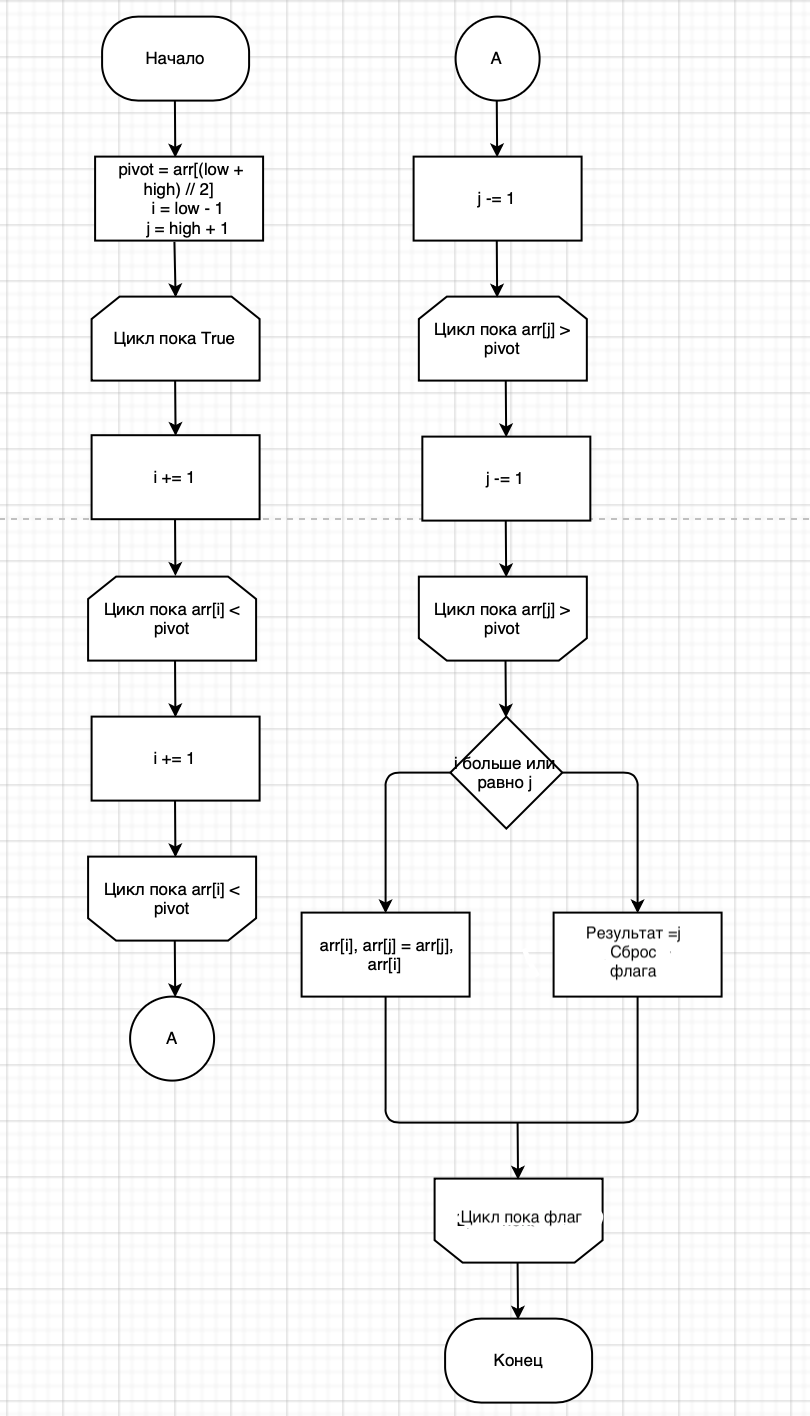
\includegraphics[scale=0.7]{Partition.png}
		
			Рис 2.5: Схема алгоритма быстрой сортировки (часть 3)
\end{center}

\section{Сравнительный анализ трудоемкости алгоритмов}

Введем модель вычислений трудоемкости алгоритма.
Пусть трудоемкость 1 у следующих базовых операций: +, -, *, /, =, ==, !=, <, <=, >, >=. Трудоемкость цикла: f цикла = f иниц + f сравн + N итер(f тела +
fинкрем + fсравн ).Трудоемкость условного перехода 1.


Алгоритм сортировки пузырьком обладает трудоемкостью \ref{eq:ref1}.

\begin{equation}
	N^2 * \left[ 
	\begin{array}{c} 
	$4 л.с.$\\
	$8.5 x.c$
	\end{array}
	\right.\\ 
	+ N * \left[ 
		\begin{array}{c} 
		$3 л.с.$\\
		$-1.5 x.c$
		\end{array}
		\label{eq:ref1}
		\right. - 4\\ 
\end{equation}

Трудоемкость квадратичная от размера массива. 

Сортировка вставками в лучшем случае, если уже отсортированный
массив: О(N).
В худшем случае, если обратно отсортированный массив: О(N^2).

Быстрая сортировка в лучшем случае: О(Nlog(N)).

В худшем случае: О(N^2).


\section{Вывод}
В данном разделе приведены схемы трех алгоритмов: сортировка пузырьком, сортировка вставками и быстрая сортировка, а так же приведена трудоемкость каждого алгоритма.

\chapter{Технологическая часть}
В данном разделе будет описана программная реализация трех алгоритмов
\section{Выбор языка программирования}
Для реализации алгоритмов методом сортировки был выбран язык программирования PYTHON как наиболее удобный и понятный для реализации алгоритмов сортировки. Для замера времени использован метод time из библиотеки time ~\cite{five}.  
\begin{lstlisting}[label=some-code,caption=Подпрограмма алгоритма сортировки "пузырьком"]
def bubble_sort(array):
    for i in range(len(array)):
        for j in range(len(array) - 1):
            if (array[j] > array[j + 1]):
                x = array[j]
                array[j] = array[j + 1]
                array[j + 1] = x        

\end{lstlisting}

\begin{lstlisting}[label=some-code,caption=Подпрограмма алгоритма сортировки вставками]
def insertion(array):
    for i in range(len(array)):
        j = i - 1
        key = array[i]
        while array[j] > key and j >= 0:
            array[j + 1] = array[j]
            j -= 1
        array[j + 1] = key
\end{lstlisting}

\begin{lstlisting}[label=some-code,caption=Подпрограмма алгоритма быстрой сортировки]
def quicksort(alist, start, end):
    if end - start > 1:
        p = partition(alist, start, end)
        quicksort(alist, start, p)
        quicksort(alist, p + 1, end)


def partition(alist, start, end):
    pivot = alist[start]
    i = start + 1
    j = end - 1

    while True:
        while (i <= j and alist[i] <= pivot):
            i = i + 1
        while (i <= j and alist[j] >= pivot):
            j = j - 1

        if i <= j:
            alist[i], alist[j] = alist[j], alist[i]
        else:
            alist[start], alist[j] = alist[j], alist[start]
            return j

\end{lstlisting}

\section{Тесты}

В данном разделе будут представлены тесты.

\begin{enumerate}
	\itemПри массиве arr = [1, 3, 5, 2, 4] 
	Сортировка пузырьком: 1 2 3 4 5
	Сортировка вставками: 1 2 3 4 5
	Быстрая сортировка: 1 2 3 4 5
	\itemПри массиве arr = [10, 9, 8, 7, 6, 5, 1, 2, 3, 4] 
	Сортировка "пузырьком": 1 2 3 4 5 6 7 8 9 10
	Сортировка вставками:  1 2 3 4 5 6 7 8 9 10
	Быстрая сортировка:  1 2 3 4 5 6 7 8 9 10
	\itemПри массиве arr = [1] 
	Сортировка "пузырьком": 1
	Сортировка вставками: 1
	Быстрая сортировка: 1 

\end{enumerate}
На рисунке 3.1 приведены результаты работы программы
\begin{center}
		\includegraphics[scale=0.7]{test.png}
		
			Рис 3.1: Снимок экрана прохождения тестов
\end{center}

Тесты пройдены успешно

\chapter{Исследовательская часть}
В данном разделе будет сделано сравнение трех алгоритмов сортировки в разных случаях
\section{Случайное заполнение массива}
\begin{center}
	\centering
	\caption{Сравнительная таблица времени выполнения (сек.) всех алгоритмов при заполнении массива случайными элементами за 50 раз}
	\begin{tabular}{|c c c c|}
		\hline
		Длина массива & Пузырек & Вставки & Быстрая сортировка  \\ [0.5ex] 
 		\hline\hline
		20 & 0.0034351  & 0.0010774  & 0.0012343\\
 		\hline
 		50 & 0.0244715& 0.0066717 & 0.0050528\\
 		\hline
 		80 & 0.0444493  & 0.0133443 & 0.0057573  \\
 		\hline
		100 & 0.0678084  & 0.0193913 & 0.0075033 \\
		\hline
		\end{tabular}
\end{center}
\newpage
График зависимости времени работы каждого алгоритма от количества элементов в последовательности(результаты приведены в (с), каждый алгоритм был выполнен 50 раз)

\begin{tikzpicture}
\begin{axis}[
    	axis lines = left,
    	xlabel = {Длина},
    	ylabel = {Время},
	legend pos=north west,
	ymajorgrids=true
]
\addplot[color=red] table[x index=0, y index=1] {bubble.dat}; 
\addplot[color=orange] table[x index=0, y index=1] {insertion.dat};
\addplot[color=blue, mark=square] table[x index=0, y index=1] {quicksort.dat};

\addlegendentry{Пузырек}
\addlegendentry{Вставки}
\addlegendentry{Быстрая сортировка}
\end{axis}
\end{tikzpicture}

\section{Лучшая ситуация}
Рассмотрим случай, когда массив длиной 50 уже изначально отсортирован(замеры произведены в (с) за 50 раз) \newline
Лучший случай для быстрой сортировки: Если в каждой итерации каждый из подмассивов будет делиться на два равных по величине массива\newline


На рисунке 4.2 показана работа алгоритмов сортировки массивов при лучшем случае.


\begin{center}
		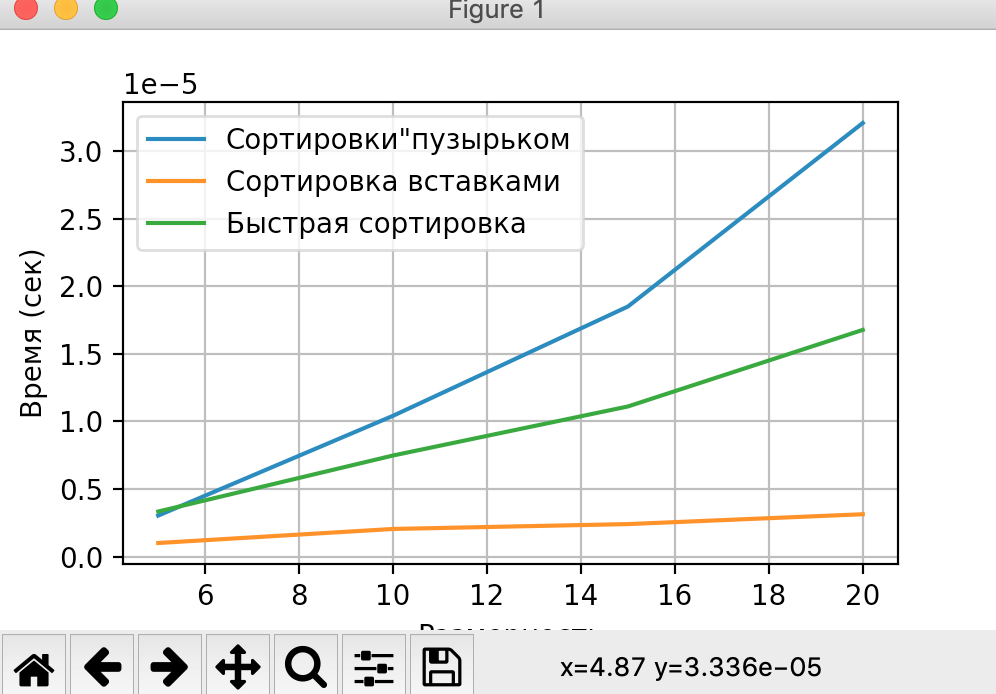
\includegraphics[scale=0.6]{Best.png}
		
			Рис 4.2: Сравнение времени выполнения алгоритмов (лучший случай)
\end{center}

\section{Худшая ситуация}
Рассмотрим случай, когда массив длиной 50 отсортирован по убыванию (замеры произведены в (с) за 50 раз) \newline
Для метода вставок наихудшим случаем является массив, отсортированный в порядке, обратном нужному, аналогично и для метода пузырька. 
Для метода быстрой сортировки худший случай наступает в 3-х ситуациях.
	\begin{enumerate}
	\item Массив уже отсортирован в том же порядке. 
	\item Массив уже отсортирован в обратном порядке. 
	\item Все элементы одинаковы (особый случай случаев 1 и 2).
	\end{enumerate}
\begin{center}
		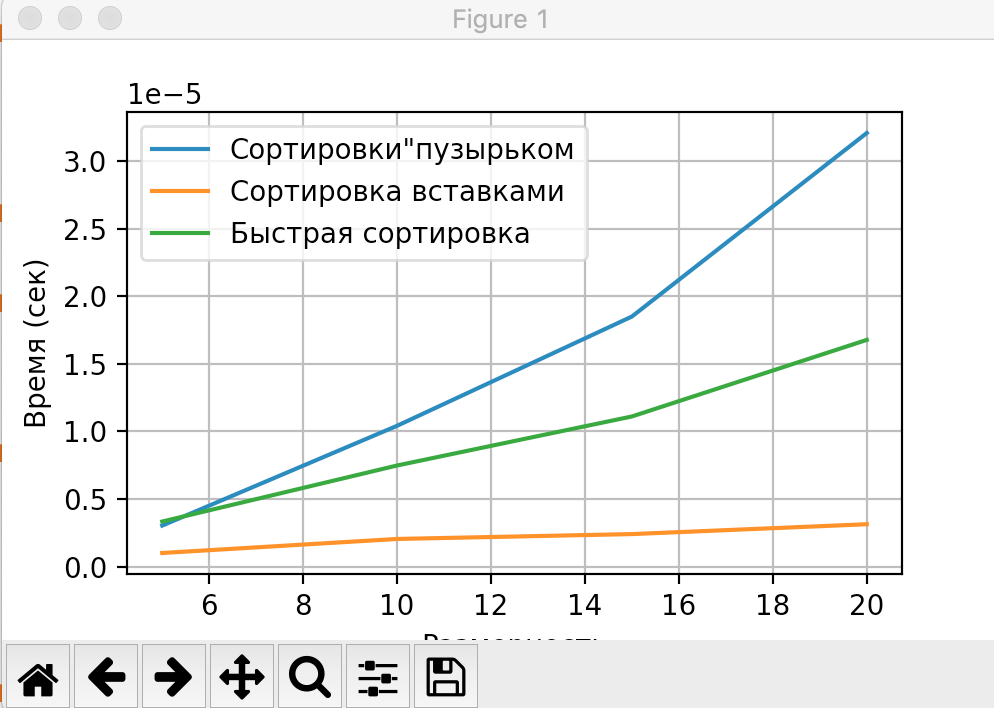
\includegraphics[scale=0.6]{Worst.png}
		
			Рис 4.3: Сравнение времени выполнения алгоритмов (худший случай)
\end{center}




\section{Вывод}
В данном разделе представлены сравнительные характеристики трех алгоритмов. Можно утверждать, что в любом случае наихудшим алгоритмом является пузырек, он работает дольше всего. Если массив изначально отсортирован, то лучшее время показал алгоритм, использующий метод вставок. В случайном случае наилучшую работоспособность показал алгоритм быстрой сортировки, так как данная ситуация встречаются чаще всего, то можно утверждать, что лучшим алгоритмом для сортировки является алгоритм быстрой сортировки.

\chapter*{Заключение}
В ходе данной лабораторной работе были изучены и программно реализованы алгоритмы сортировок(пузырек, вставка, метод быстрой сортировки). Сделан вывод, что в худшем случае все эти алгоритмы имеют квадратичную сложность. В остальных случаях наилучший результат показал алгоритм быстрой сортировки. Так же хотелось бы отметить, что алгоритм пузырька прост для написания, в отличие от алгоритма быстрой сортировки. Алгоритм пузырек проигрывает по времени остальным алгоритмам, следовательно, является самым медленным. \newline
В заключении достигнута поставленная цель и решены следующие задачи.

\begin{enumerate}
\item Изучен и программно реализован алгоритм сортировки "пузырьком".
\item Изучен и программно реализован алгоритм сортировки вставками.
\item Изучен и программно реализован алгоритм быстрой сортировки.
\item Оценена трудоемкость вышеперечисленных алгоритмов.
\item Сделан сравнительный анализ по затрачиваемым ресурсам (времени) компьютера на реализацию каждого рассмотренного алгоритма.
\end{enumerate}

\begin{thebibliography}{9}

\addcontentsline{toc}{chapter}{Литература}
 
	\bibitem{one}
Т. Кормен, Ч. Лейзерсон, Р. Ривест, К. Штайн - Алгоритмы. Построение и анализ. Издание 3-е
 
	\bibitem{two}
	Алгоритмы: разработка и применение
Авторы: Джон Клейнберг, Эва Тардос.
Год издания: 2016.

 
	\bibitem{free}  
	Введение в анализ алгоритмов
Автор: Майкл Солтис. Год издания: 2019.
	
	\bibitem{four}
	Vijay V. Vazirani, «Approximation Algorithms»  — о том, как быстро находить достаточно хорошие решения для трудных оптимизационных задач.
	
	\bibitem{five}
	Совершенный алгоритм. Основы
Автор: Тим Рафгарден. Год издания: 2019.
	
\end{thebibliography}


\end{document}